\section{Project Goals}

\par Goal-oriented-capture allowed the team to determine the goals and requirements for the project from all stakeholders . These were found to include goals relating to both neurodynamic and computational performance. Figure \ref{goc} is a visual representation of the process the team undertook in order to fully formulate the specification. 

\begin{figure}[b!]
  \centering
    \makebox[\textwidth]{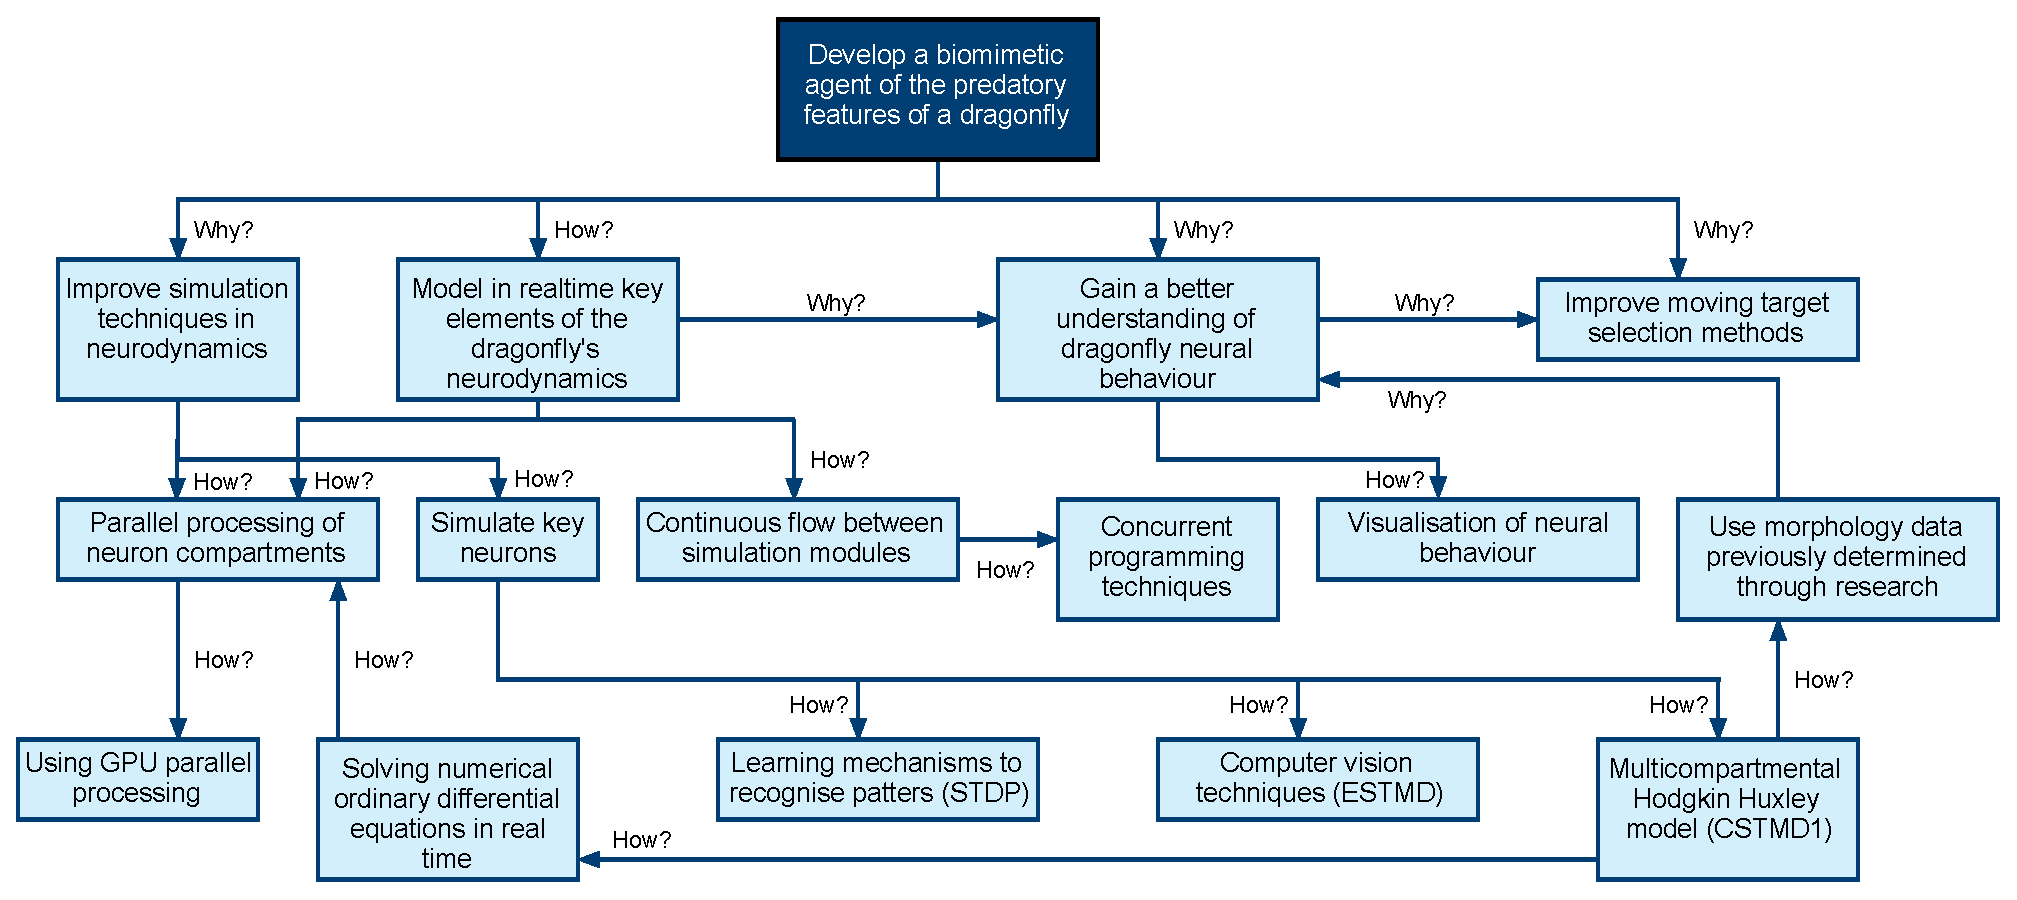
\includegraphics[width=\textwidth]{RequirementsCapture.eps}}
  \caption{Goal-oriented-capture}
  \label{goc}
\end{figure}

\newpage

\par The goal oriented capture coupled with discussions with our supervisors over the extent of existing research allowed us to estimate the level of complexity for each component and split their functionality into three stages of development. The resulting specification is shown in Table \ref{table:req}.

\begin{table}[h!]
\begin{tabularx}{\hsize}{c | c |X}
\multirow{8}{*}{\rotatebox[origin=c]{90}{Minimal}} & A1 & Develop an efficient implementation of a multicompartmental Hodgkin-Huxley neuron model \\
& A2 & Apply this model to create a CSTMD1 simulation \\
& A3 &Integration of ESTMD, STPD and RL with the CSTMD1 neuron(s) into a continuous flow simulation \\
& A4 &2D environment in which the agent will attempt to capture prey \\
& A5 &Implement and integrate a motor module which moves the dragonfly within the environment and automatic system\\
\hline
\multirow{5}{*}{\rotatebox[origin=c]{90}{Full}}
& B1 & Providing a transparent interface in order to understand the characteristics of each module \\
& B2 & Create and display a visualisation of agent's neural behaviour \\
& B3 & The CSTMD1 module exhibiting all theoretically expected features\\
& B4 & Comparison of our own simulation with 3$^{rd}$ party simulators including NEURON \\
& B5 & The connected modules should be able to run in an approximation of real-time\\
\hline
\multirow{5}{*}{\rotatebox[origin=c]{90}{Extensions}}
& C1 & Create a user interface for the virtual simulation environment \\
& C2 & Implement with real-time input from camera \\
& C3 & Extend the enviroment and motor controller to improve realism \\
& C4 &Implement on a simple physical robot or quad-copter \\ 
\end{tabularx}
\caption{Project Specification/Requirements}
\label{table:req}
\end{table}